\section{Coarse-grained simulations}

\begin{figure}[ht]
  \begin{centering}
  \adjustbox{minipage=1.3em,valign=t}{\subcaption{}\label{sfig:testa}}%
  \begin{subfigure}[t]{\dimexpr.4\linewidth-1.3em\relax}
  \centering
  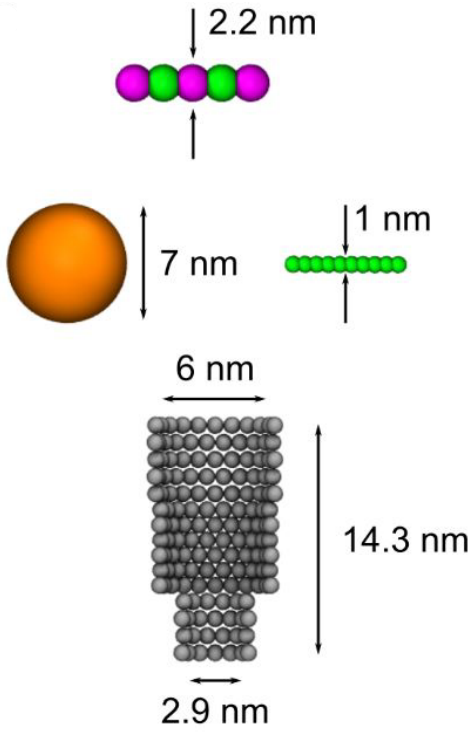
\includegraphics[width=0.9\linewidth,valign=t]{Figures/Stefanos1.png}
  \end{subfigure}%
  \adjustbox{minipage=1.3em,valign=t}{\subcaption{}\label{sfig:testb}}%
  \begin{subfigure}[t]{\dimexpr.5\linewidth-1.3em\relax}
  \centering
  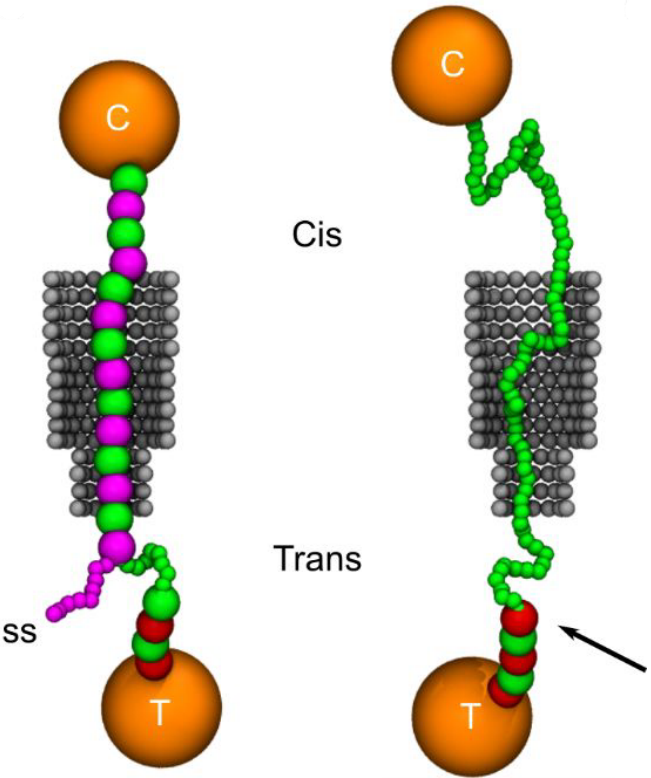
\includegraphics[width=0.9\linewidth,valign=t]{Figures/Stefanos2.png}
  \end{subfigure}
  \caption{This is a figure}
  \label{fig:test}
  \end{centering}
\end{figure}

to investigate the typical conformations of rotaxanes-ds and ss at zero bias. This
approach is justified by the long time scales ofinterest, and the high salt concentration
of the solution (2 M KCl). A numerical analysis ofthe electrostatic energies, using the
Poisson−Boltzmann equations, indeed indicates that electrostatic DNA-nanopore
interactions are weak and repulsive (Figures S4 and S5 in Section S8). These interactions
were accounted for by properly adjusting the dimensions of the pore

the fact that the piston operates at both positive and negative applied bias suggests
that the electrophoretic bias is not necessary for its functioning. Indeed, simulations
indicate that entropy plays a more central role.

LAMMPS.

Discuss semiflexible bead-and-spring model DNA + repulsive LJ interactions to simulate
excluded volume interactions.

Each spherical ssDNA (dsDNA) bead represented 1 nt (ssDNA) or 5 bp (dsDNA), had a
diameter of 1 nm (ssDNA) or 2.2 nm (dsDNA) and an average bond distance of 0.68 nm
(ssDNA) or 1.7 nm (dsDNA).

ClyA consisted of three connected open cylinders, with diameters 6 nm, 5.5 nm and 2.9 nm
from the cis- to the trans-side, following the geometry reported in []
%Bell, N. A.; Engst, C. R.; Ablay, M.; Divitini, G.; Ducati, C.; Liedl, T.; Keyser, U. F.
%DNA Origami Nanopores. Nano Lett. 2012, 12 (1), 512−517. (4)
The latter value is somewhat smaller than the reported one (3.3 nm), accounting for the
electrostatic repulsion between DNA and the negatively-charged trans-entry.
The lipid bi layer in which the pore is embedded is simulated by a reflective boundary at
the lower entrance of the nanopore interacting only with the neutravidin beads.

Neutravidin was modeled as a sphere of diameter 7 nm, attached to the two ends of the
rotaxane. The motivation of this size was done by simulating the neutravidin bead
together with the ClyA nanopore and fitting the size of the neutravidin bead so that it
could be caputed in the lumen of the nanopore, as is seen in experiments.


The bond strength is chosen to be, by transforming the equation for persistence length
kSsDNA = persistenceSsDNA * boltzmann * temperature / lengthNt
kDsDNA = persistenceDsDNA * boltzmann * temperature / lengthBp
For the description of ssDNA and dsDNA, with persistence lengths 2.2 nm and 45 nm,
respectively.

$k_{bond} = l_p * k_{bt} * T / \langle a \rangle$
Kuhn segments for ssDNA en dsDNA are different!

Gaussian probably distribution of the beads, i.e. the beads show ideal chain behaviour.
Equipartition theorem.

$k_{bond} = 3 k_b T / \langle a \rangle$

Langevin integrator is used As is common in simula- tions of coarse-grained models. As is
common practice in MD simulations, the diffusion coefficient of the oxDNA strand is
chosen larger then the value of physical DNA. This is done to speed up the simulations,
while ensuring its physical accuracy.

Discuss limits of the model. Limited accuracy of the CG model since it does not caputre
the full structure of DNA accurately. For example the double helix structure is note
captured. Another consequence is that the DNA hybridisation can not be simulated using
this model, since both ssDNA nucleotides and dsDNA basepairs are represented by simple
beads. To further analyse and understand the operation cycle of the nanopiston a more
accurate CG model is needed.
